
\chapter{X的相关配置}
\label{chap:xconfiguration}

\rule[0pt]{\textwidth}{0.1pt}

\section{什么是X}
\label{chap:xconfiguration:whatis}
千万年前……计算机的终端只包含一个屏幕和键盘,就没有其它东西了。那时候,
鼠标是个稀少的东西,终端下的操作都是菜单驱动的。上帝说,要有图形接口,
于是就有了图形用户接口(GUI),之后,世界发生了巨大的变化。当今的用户
都习惯于在屏幕上移移鼠标,点点图标,运行的程序也带有漂亮的图片和动画。
但UNIX是在GUI之前诞生的,所以UNIX中的GUI有点事后诸葛的味道。在很长一段
时期,人们都在毫无图形界面支持的环境下工作,但现在的Linux用户恐怕没有人
不是工作在一个美仑美涣的可指点的GUI环境了吧,这些GUI都运行在
\textit{X\textbf{(7)}}之下。

那么,什么是X?它是一个带有图标的桌面吗?还是说是菜单?难道是窗口管理
器?它会为一些点作标记吗\footnote{Does it mark the spot,不懂怎么翻
  译。}?天空中一记响亮的回声:不!GUI由很多部分组成,X只是其中最基本
的部分。X是一个从鼠标、键盘或是其它设备中获取输入的软件。X是告诉显卡应
该怎么操作的软件。简单地说,X就是一个以图形为目的与系统硬件交流的软件;
而其它所有的图形软件只和X进行对话。

我们先停一下来讨论X的命名,X只是那一打名字中的一个。它还被叫作X11、
xorg、the X Window System、X Window、X11R6, X Version 11以及其它的一
些名字。无论你听到的是哪个,只要把它理解为X就行了。

从Slackware-10.0开始,Slackware中的X Window环境就是由Xorg提供的。所谓
的X,就是为用户提供图形接口,它与操作系统是独立的,在这点上与Windows或
MacOS不同。

X Window System 是由许多运行在用户空间的程序组成的。最主要的两大部分就
是X服务器和窗口管理器。X服务器提供了与视频硬件相互作用的函数,所以是专
门针对系统设计的。窗口管理器位于X服务器之上,为用户提供用户接口。采用
这个架构的优点就在于我们可以拥有多种用户接口,而这只要通过选择不同的窗
口管理器就能实现。

\section{设置X服务器}
\label{chap:xconfiguration:configuration}
曾经有这么一段时间,那时配置X是困难并且痛苦的过程,成百上千的显示器都
因此``冒烟''了。而现在,X已经很人性化了。事实上,多数用户根据不要需要
去配置X,Slackware会自动检测并做出正确的设置。然而,还是有一些计算机不
会被正确地识别,因此需要一些额外的手工设置。

之前(起码在Slackbook 2.0的年代),X的配置文件为
\path{/etc/X11/xorg.conf}文件,并且如果你创建了这个文件,X会尊重你在该
文件中做出的任何配置,即采用这些配置。幸运的是,从XOrg 1.6.3开始,X不
需要\path{/etc/X11/xorg.conf}文件就能正常地工作。如果因为某个不为人知
的原因,你需要为X做一些设置,我们建议你也不要使用这个文件,这个文件已
经较为过时,并且它的灵活性很差。现在我们采用的是在
\path{/etc/X11/xorg.conf.d/}文件夹来对X进行配置。X在启动时会读取该文件
夹中的配置文件,这就使得我们可以将对X的配置分为几个部分,从而方便管理。
注意,\path{/etc/X11/xorg.conf.d/}文件夹中的配置文件的文件名要以
\path{.conf}结尾。例如,下面是我的笔记本上的
\path{/etc/X11/xorg.conf.d/synaptics.conf}文件的内容。

\begin{Verbatim}[frame=single, commandchars=\\\{\}]
darkstar:~\$ \textbf{cat /etc/X11/xorg.conf.d/synaptics.conf}
Section "InputDevice"
    Identifier      "Synaptics Touchpad"
    Driver          "synaptics"
    Option          "SendCoreEvents"        "true"
    Option          "Device"                "/dev/psaux"
    Option          "Protocol"              "auto-dev"
    Option          "SHMConfig"             "on"
    Option          "LeftEdge"              "100"
    Option          "RightEdge"             "1120"
    Option          "TopEdge"               "50"
    Option          "BottomEdge"            "310"
    Option          "FingerLow"             "25"
    Option          "FingerHigh"            "30"
    Option          "VertScrollDelta"       "20"
    Option          "HorizScrollDelta"      "50"
    Option          "MinSpeed"              "0.79"
    Option          "MaxSpeed"              "0.88"
    Option          "AccelFactor"           "0.0015"
    Option          "TapButton1"            "1"
    Option          "TapButton2"            "2"
    Option          "TapButton3"            "3"
    Option          "MaxTapMove"            "100"
    Option          "HorizScrollDelta"      "0"
    Option          "HorizEdgeScroll"       "0"
    Option          "VertEdgeScroll"        "1"
    Option          "VertTwoFingerScroll"   "0"
EndSection
\end{Verbatim}
把对X配置的每个小节者单独保存为一个文件,能更好地对X的配置文件进行管理。
你也可以查看\path{/usr/share/X11/xorg.conf.d},查看Slackware对X的一些
默认配置文件。


\subsection{生成xorg.conf}
\label{chap:xconfiguration:configuration:generateXorg}
尽管上面我们已经介绍了如何对X进行配置,但主要还是介绍X的配置文件的布局,
且体的配置方法还没说明。首先,关于X配置文件的语法请参见Xorg的man手册,
此处不再介绍,这里要介绍的是Slackware中提供的两个自动生成配置文件的工
具:Xorg与xorgsetup。

运行命令
\begin{Verbatim}[frame=single, commandchars=\\\{\}]
darkstar~# \textbf{Xorg -configure} # 或
darkstar~# \textbf{X-configure} 
\end{Verbatim}
则Xorg会自动检测当前机器的硬件,并在\path{/root}目录下生成一个
\path{xorg.conf.new}文件,我们可以先用如下命令对该文件进行测试:
\begin{Verbatim}[frame=single, commandchars=\\\{\}]
darkstar~# \textbf{Xorg -config /root/xorg.conf.new -retro}
\end{Verbatim}
如果之后屏幕上出现一个``X''的鼠标图标,并能正常移动,那么一般说足以说
明该xorg.conf文件是正确的,之后可以将其复制为\path{/etc/X11/xorg.conf},
采用古老的方法配置X,或者将该文件中的需要的某些部分复制为新的文件,放
入\path{/etc/X11/xorg.conf.d}文件夹中,会用同样的效果。当然,就是上面
提到的,现在建议采用第二种形式。

这是一个很方便的方法,但在Slackware中,还保留着一个脚本配置工具,它就
是\texttt{xorgsetup},它是一个脚本,以\texttt{root}权限运行,会有一些选
项让用户选择,再根据对硬件的检测生成正确的配置文件。对于新手进行配置也
是很有帮助的,生成配置文件后的用法就不再赘述。

\section{选择窗口管理器}
\label{chap:xconfiguration:select}
Slackware中包含了许多不同的窗口管理器及桌面环境。窗口管理器是一种用于
在屏幕上画出应用程序窗口、改变窗口大小及类似工作的一个程序。而桌面环境
除了包含一个窗口管理器外,还包含任务栏、菜单、图标及一些其它的东西。
Slackware中包含了KDE及XFCE桌面环境以及其它的一些窗口管理器。使用哪一个
完全取决于你的喜好,但一般而言,窗口管理器比桌面环境要快,所以更适合于
那些缺内存、CPU慢的老机器。桌面环境对习惯使用Windows的用户更为友好。

\subsection{xinitrc}
\label{chap:xconfiguration:select:xinitrc}
\texttt{xinit\textbf{(1)}}是真正启动X的程序;它由
\texttt{startx\textbf{(1)}}调用,所以你可能不会注意到它的存在(也不需
要注意到)。但它的配置文件决定了X启动时,运行哪个程序(尤其包括了使用哪个窗口管
理器)。\texttt{xinit}首先检查主目录下是否有\path{.xinitrc}文件,如果
有,就使用它进行启动;否则就使用\path{/etc/X11/xinit/xinitrc}(系统默
认)文件进行启动。下面是\texttt{xinitrc}文件的一个例子:
\begin{Verbatim}[frame=single, commandchars=\\\{\}]
#!/bin/sh
# \$XConsortium: xinitrc.cpp,v 1.4 91/08/22 11:41:34 rws Exp \$
userresources=\$HOME/.Xresources
usermodmap=\$HOME/.Xmodmap
sysresources=/usr/X11R6/lib/X11/xinit/.Xresources
sysmodmap=/usr/X11R6/lib/X11/xinit/.Xmodmap

# merge in defaults and keymaps
if [ -f \$sysresources ]; then
xrdb -merge \$sysresources
fi
if [ -f \$sysmodmap ]; then
xmodmap \$sysmodmap
fi
if [ -f \$userresources ]; then
xrdb -merge \$userresources
fi
if [ -f \$usermodmap ]; then
xmodmap \$usermodmap
fi
# start some nice programs
twm \&
xclock -geometry 50x50-1+1 \&
xterm -geometry 80x50+494+51 \&
xterm -geometry 80x20+494-0 \&
exec xterm -geometry 80x66+0+0 -name login
\end{Verbatim}

上面所有的``if''语句的作用是整合在其它配置文件中的配置信息。该文件有趣
的地方是文件末尾,这里我们运行了很多程序。X会话会开启
\texttt{twm\textbf{(1)}}窗口管理器、一个时钟及三个虚拟终端。注意到在最
后一个\texttt{xterm}前的\texttt{exec},它的作用是用最后一行的
\texttt{xterm\textbf{(1)}}命令替换当前运行的shell(即当前执行
\texttt{xinitrc}脚本的shell),当用户从那个\texttt{xterm}中退出时,整
个X会话就结束了。

要定制自己的X启动脚本,只要将\path{/etc/X11/xinit/xinitrc}文件复制到
\path{~/.xinitrc}文件并进行修改,随意替换那些运行程序的行。例如我们
xinitrc文件最后几行就是:
\begin{Verbatim}[frame=single, commandchars=\\\{\}]
# Start the window manager
exec startkde
\end{Verbatim}
注意,在\path{/etc/X11/xinit}文件夹中的那些\path{xinitrc.*}文件对应启
动了相应的窗口管理器及GUI。我们也可以直接拿来使用。

\subsection{xwmconfig}
\label{chap:xconfiguration:select:xwmconfig}
由于Slackware中安装的窗口管理器和桌面环境比较多,配置起来也相对麻烦一
些,所以Slackware中包含了一个名为\texttt{xwmconfig}的程序,用来选择窗
口管理器。运行如下:
\begin{Verbatim}[frame=single, commandchars=\\\{\}]
darkstar~\% \textbf{xwmconfig}
\end{Verbatim}

\begin{figure}[htpb]
  \centering
  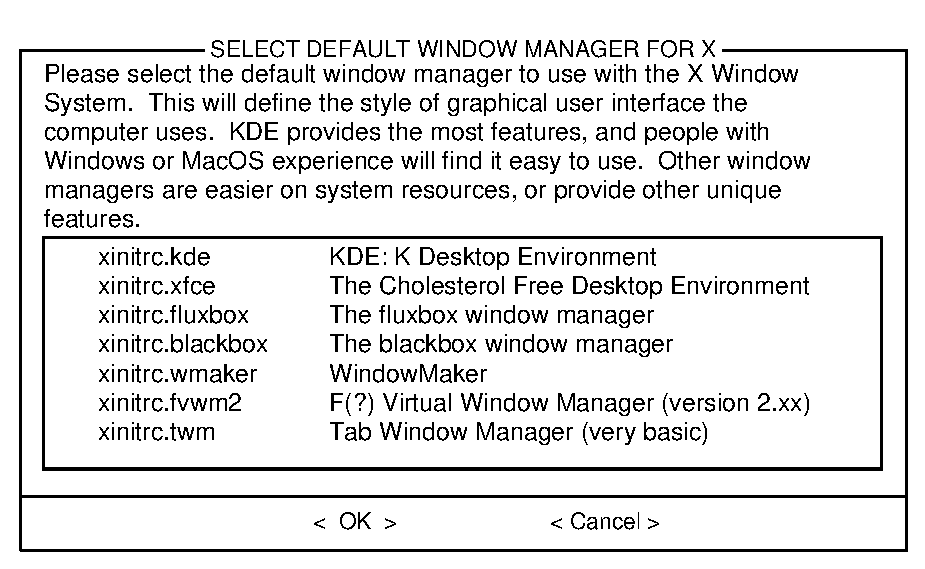
\includegraphics[width=0.8\textwidth]{images/installation/setup-xwmconfig.eps}
  \caption{使用xwmconfig选择桌面}
  \label{fig:selectX-xwmconfig}
\end{figure}

运行之后会显示当前安装的所有窗口管理器的列表,选择自己想用的即可。安装
过程中也是使用此程序选择窗口管理器。因为每个人的风格不同,也没有必要都
选择默认的。

之后启动X就万事OK了。

\section{启动进入图形界面}
\label{chap:xconfiguration:bootInX}
默认情况下,Slackware启动后会显示一个虚拟终端,并提示登陆。这对于大多
数用户已经足够满足要求了。如果你要运行的是命令行程序,那么登陆后直接在
终端中运行即可,如果你想运行X,那么登陆后运行\texttt{startx}就可以启动
X了。但如果我们的工作几乎是在图形界面下的呢?这种情况下,直接登陆GUI界
面会不会更方便一点呢?幸运的是,这种想法很容易就能达成了。

Slackware使用System V的init系统,这就使得管理员能启动进入或临时改变为
某个运行级别。事实上,关机也只是改变运行级别而已。运行级别的内容也比较
复杂,这里就不深入讨论了。

运行级别是通过\texttt{inittab\textbf{(5)}}配置的。最常用的是第3级
(Slackware默认的运行级别)以及第4级(GUI)。如果想让Slackware启动后进
入GUI界面,那么只要用文本编辑器(可以考虑先看看介绍vi或emacs的章节
% TODO:add link
)打开\path{/etc/inittab}文件进行修改即可。在文件中找到这些行:
\begin{Verbatim}[frame=single, commandchars=\\\{\}]
# These are the default runlevels in Slackware:
#   0 = halt
#   1 = single user mode
#   2 = unused (but configured the same as runlevel 3)
#   3 = multiuser mode (default Slackware runlevel)
#   4 = X11 with KDM/GDM/XDM (session managers)
#   5 = unused (but configured the same as runlevel 3)
#   6 = reboot

# Default runlevel. (Do not set to 0 or 6)
id:3:initdefault:
\end{Verbatim}
该文件中(大多数配置文件也是如些),所有在\#号之后的内容都是注释,
\texttt{init\textbf{(8)}}不会解释这些内容。即使你对initab不理解也没关
系,因为很多老手也不理解。我们感兴趣的只有最后一行,把其中的3改成4就可
以了,之后重启就完成任务了。
\begin{Verbatim}[frame=single, commandchars=\\\{\}]
# These are the default runlevels in Slackware:
#   0 = halt
#   1 = single user mode
#   2 = unused (but configured the same as runlevel 3)
#   3 = multiuser mode (default Slackware runlevel)
#   4 = X11 with KDM/GDM/XDM (session managers)
#   5 = unused (but configured the same as runlevel 3)
#   6 = reboot

# Default runlevel. (Do not set to 0 or 6)
id:4:initdefault:
\end{Verbatim}

改完之后,Slackware就会启动进入第4个运行级别,并且运行
\path{/etc/rc.d/rc.4}文件(之前的第
\ref{sec:systemConfig:systemOverview:etcRcd:runlevelInit}节文件系统布局
中介绍过了)。该文件会启动X并调用我们选择的登陆管理器。那么登陆管理器
在哪选择的呢?有好几种方法,我们会在看完\path{rc.4}的内容后进行介绍。
\begin{Verbatim}[frame=single, commandchars=\\\{\}]
# Try to use GNOME’s gdm session manager:
if [ -x /usr/bin/gdm ]; then
exec /usr/bin/gdm -nodaemon
fi
# Not there? OK, try to use KDE’s kdm session manager:
if [ -x /opt/kde/bin/kdm ]; then
exec /opt/kde/bin/kdm -nodaemon
fi
# If all you have is XDM, I guess it will have to do:
if [ -x /usr/X11R6/bin/xdm ]; then
exec /usr/X11R6/bin/xdm -nodaemon
fi
\end{Verbatim}
正如我们看到的,\path{rc.4}先检查\texttt{gdm}的存在与否及是否可执行,如
果存在且可执行则执行gdm,之后检查\texttt{kdm},最后是\texttt{xdm}。选
择登陆管理器的一个方法就是用\texttt{removepkg}把不想要的管理器删除。关
于\texttt{removepkg}的内容请参见第章。%TODO:REF chap18

当然,我们也可以把不想使用的管理器的可执行权限取消了。\texttt{chmod}命
令会在第章中介绍。%TODO: REF chap19
\begin{Verbatim}[frame=single, commandchars=\\\{\}]
darkstar~# \textbf{chmod -x /usr/bin/gdm}
\end{Verbatim}

最后,可以把不想使用的窗口管理器在\texttt{rc.4}文件中注释了。
\begin{Verbatim}[frame=single, commandchars=\\\{\}]
# Try to use GNOME’s gdm session manager:
# if [ -x /usr/bin/gdm ]; then
# exec /usr/bin/gdm -nodaemon
# fi

# Not there? OK, try to use KDE’s kdm session manager:
if [ -x /opt/kde/bin/kdm ]; then
    exec /opt/kde/bin/kdm -nodaemon
fi

# If all you have is XDM, I guess it will have to do:
if [ -x /usr/X11R6/bin/xdm ]; then
    exec /usr/X11R6/bin/xdm -nodaemon
fi
\end{Verbatim}
上面,我们把gdm的内容加了注释,即使gdm存在并可执行,shell也不会对它进行
检测。
%%% Local Variables: 
%%% mode: latex
%%% TeX-master: "../SlackGuide"
%%% End: 
